\chapter{図表}\label{chap:chapter3}

\begin{table}[b]
    \centering
    \caption{MID-360 Specifications}
    \label{table:mid360_spec}
    \begin{tabular}{| p{0.35\textwidth} | p{0.6\textwidth} |}
    \hline
    Model & MID-360 \\
    Laser Wavelength & 905 nm \\
    Laser Safety\textsuperscript{1} & Class 1 (IEC60825-1:2014) Eye Safety \\
    Detection Range @100 klx & 40 m @ 10 \% reflectivity \\
                                    & 70 m @ 80 \% reflectivity \\
    Close Proximity Blind Zone\textsuperscript{2} & 0.1 m \\
    FOV & Horizontal: 360$^\circ$, Vertical: -7$^\circ$ to 52$^\circ$ \\
    Range Precision (1$\sigma$)\textsuperscript{3} & $\leq 2\text{ cm}\textsuperscript{4}$ (@10 m) \\
                                                            & $\leq 3\text{ cm}\textsuperscript{5}$ (@0.2 m) \\
    Angular Precision (1$\sigma$) & $< 0.15^\circ$ \\
    Point Rate & 200,000 points/s (first return) \\
    Frame Rate & 10 Hz (typical) \\
    Data Port & 100 BASE-TX Ethernet \\
    Data synchronization & IEEE 1588-2008 (PTPv2), GPS \\
    Anti-Interference Function & Available \\
    False Alarm Rate @100 klx\textsuperscript{6} & $< 0.01$ \% \\
    IMU & Built-in IMU Model: ICM40609 \\
    Operating Temperature\textsuperscript{7} & -4$^\circ$F to 131$^\circ$F (-20$^\circ$C to 55$^\circ$C) \\
    IP Rating & IP67 \\
    Power\textsuperscript{8} & 6.5 W (average) \\
    Power Supply Voltage Range & 9--27 V DC \\
    Dimensions & 65$\times$65$\times$60 mm \\
    Weight & 265 g \\
    \hline
    \end{tabular}
\end{table}

\clearpage

\textbf{Fig.~\ref{fig:topic_comm}}にROS 2 のトピック通信の画像を示す.

\begin{figure}[t]
    \centering
    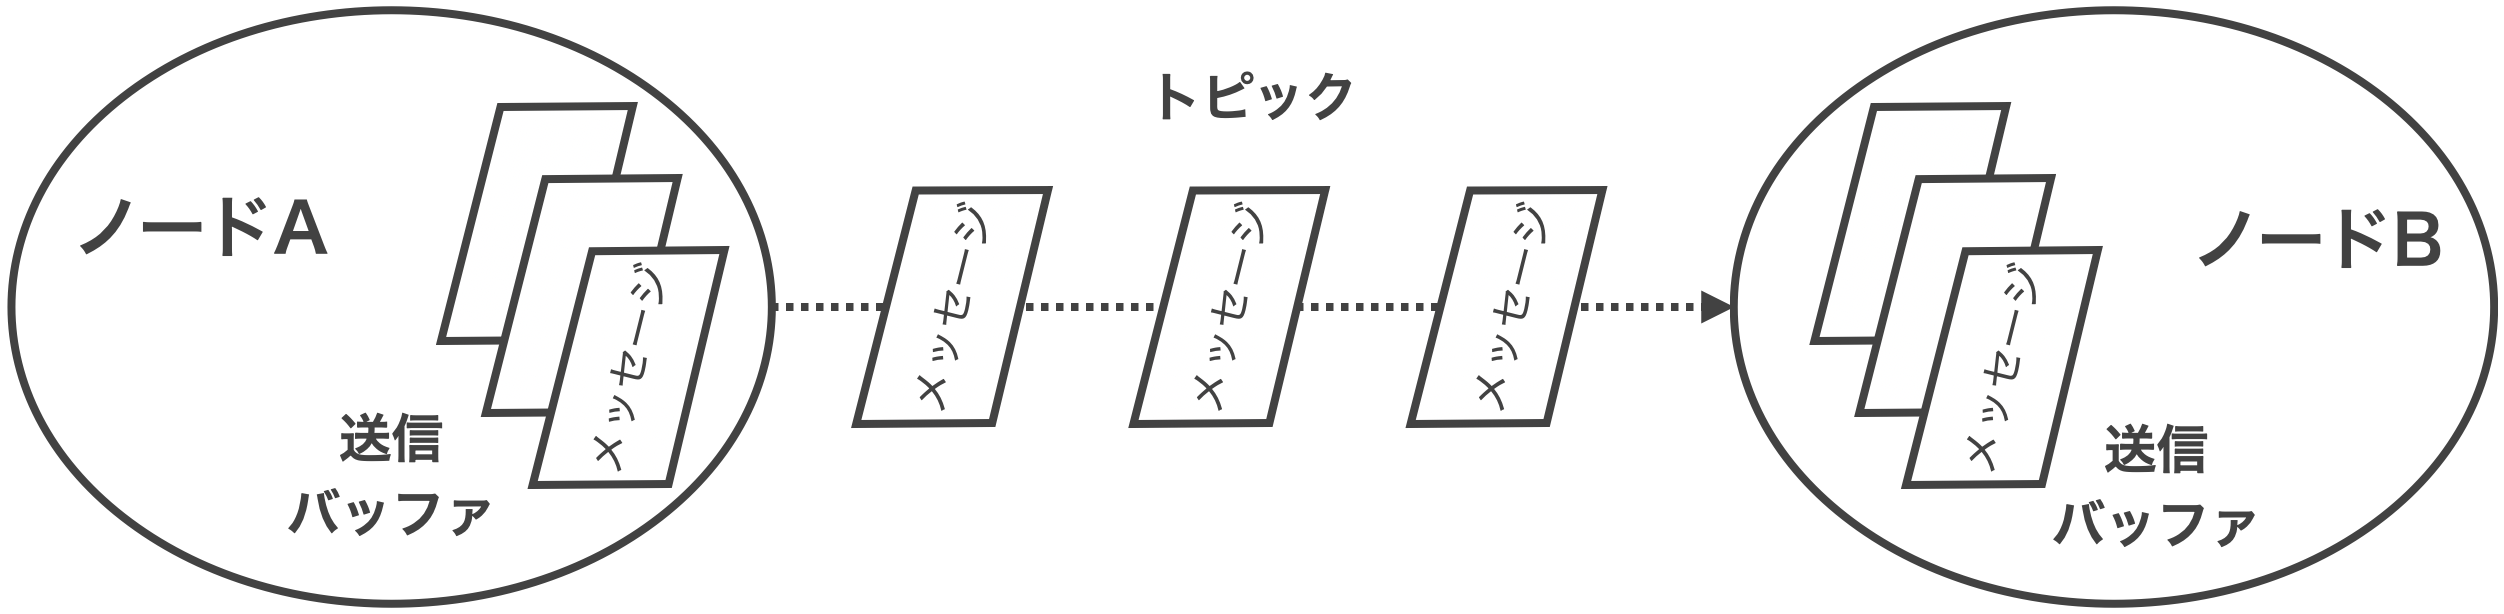
\includegraphics[width=0.8\textwidth]{fig/topic_comm.png}
    \caption{ROS 2 communication: Topic communiacation }
    \label{fig:topic_comm}
\end{figure}
